%#####################################################################################################################
% Datei	: 	Anhang.tex
% Autor	:	Byron Worms
%#####################################################################################################################
\begin{appendices}
\chapter{Abbildungen}
\label{chap:anhang_abbildungen}
\hideInContents
% Abbildung: Screenshots
\section{Screenshots}
%---------------------------------------------------------------------------------------------------------------------
\subsection{Hauptmen�}
\begin{figure}[H]
	\begin{center}
		\fbox{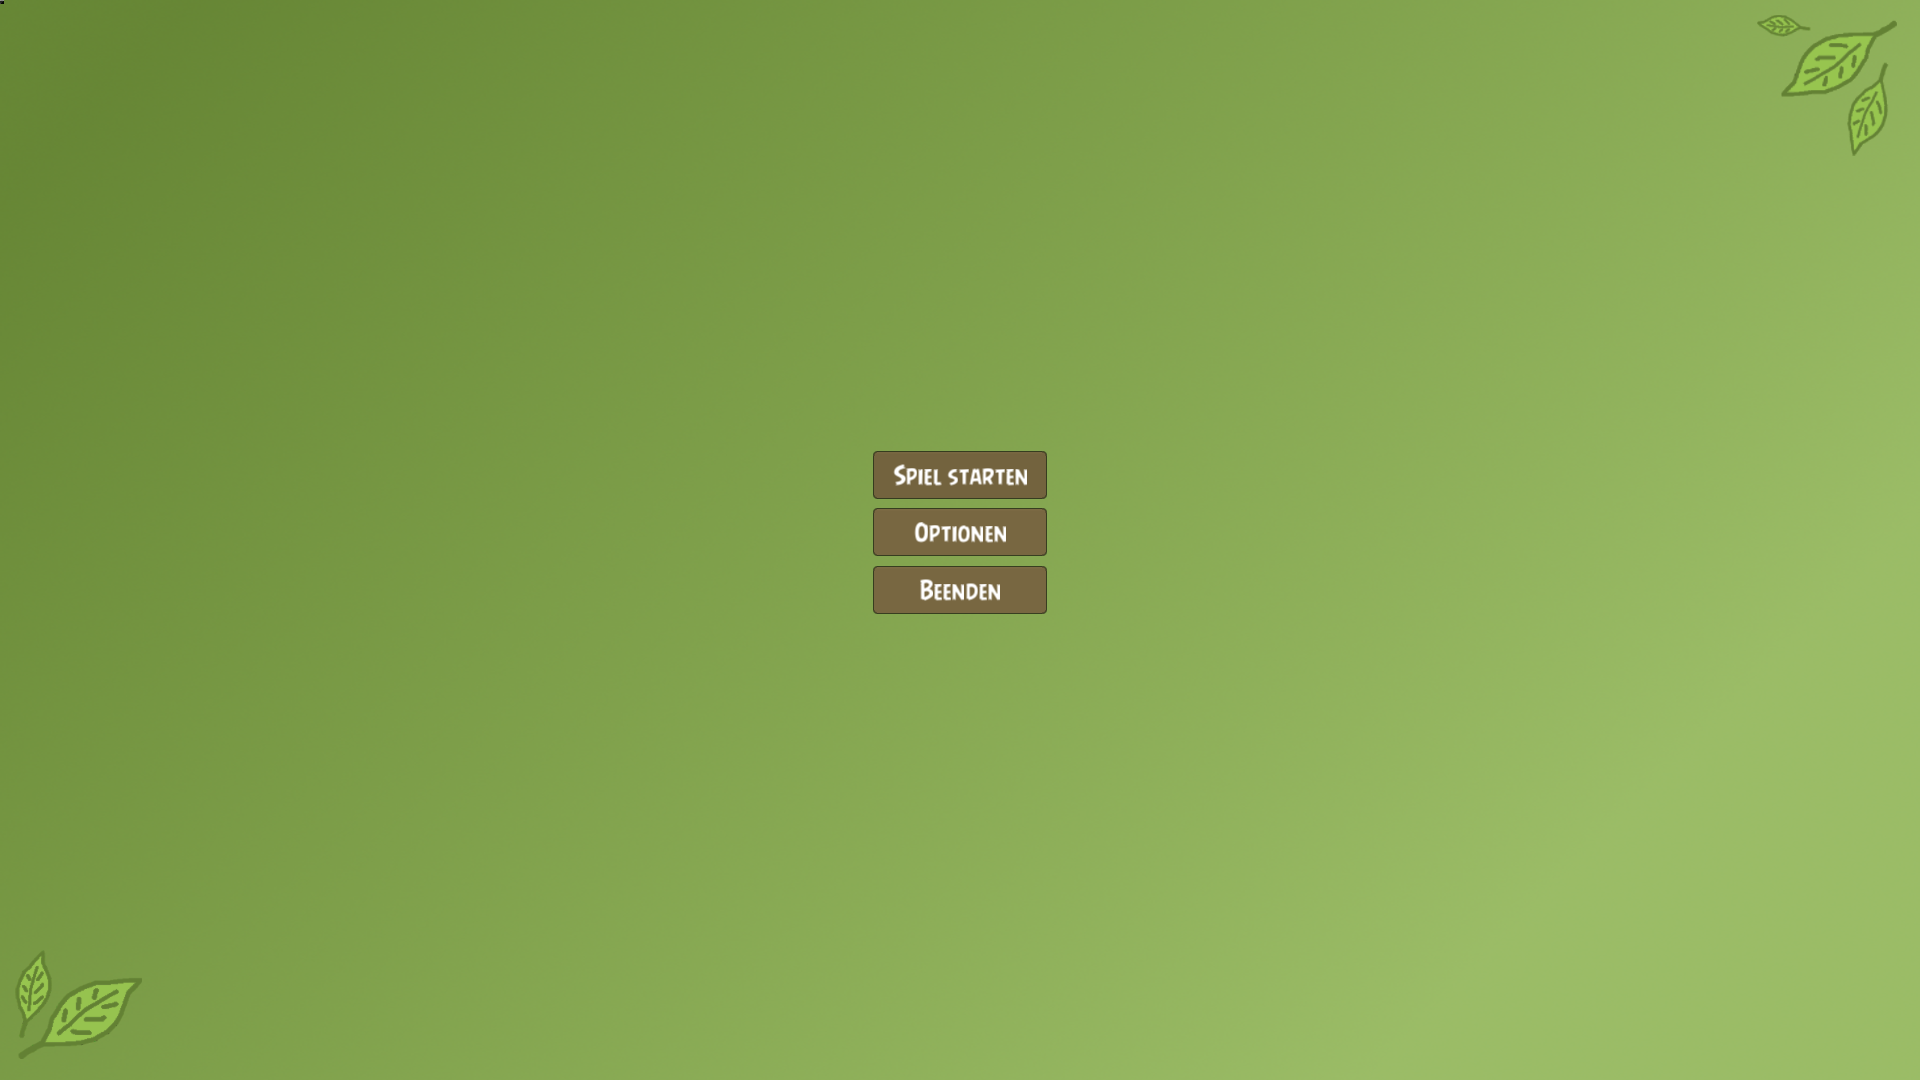
\includegraphics[page=1,width=0.98\linewidth]{Inhalt/Anhang/Screenshots/screenshot_0.png}}
	\end{center}	
	\caption[Hauptmen�]{Hauptmen� (Eigene Darstellung)}
	\label{fig:anhang_screenshots_menu}
\end{figure}
%---------------------------------------------------------------------------------------------------------------------
\subsection{Analyse--Level}
\begin{figure}[H]
	\begin{center}
		\fbox{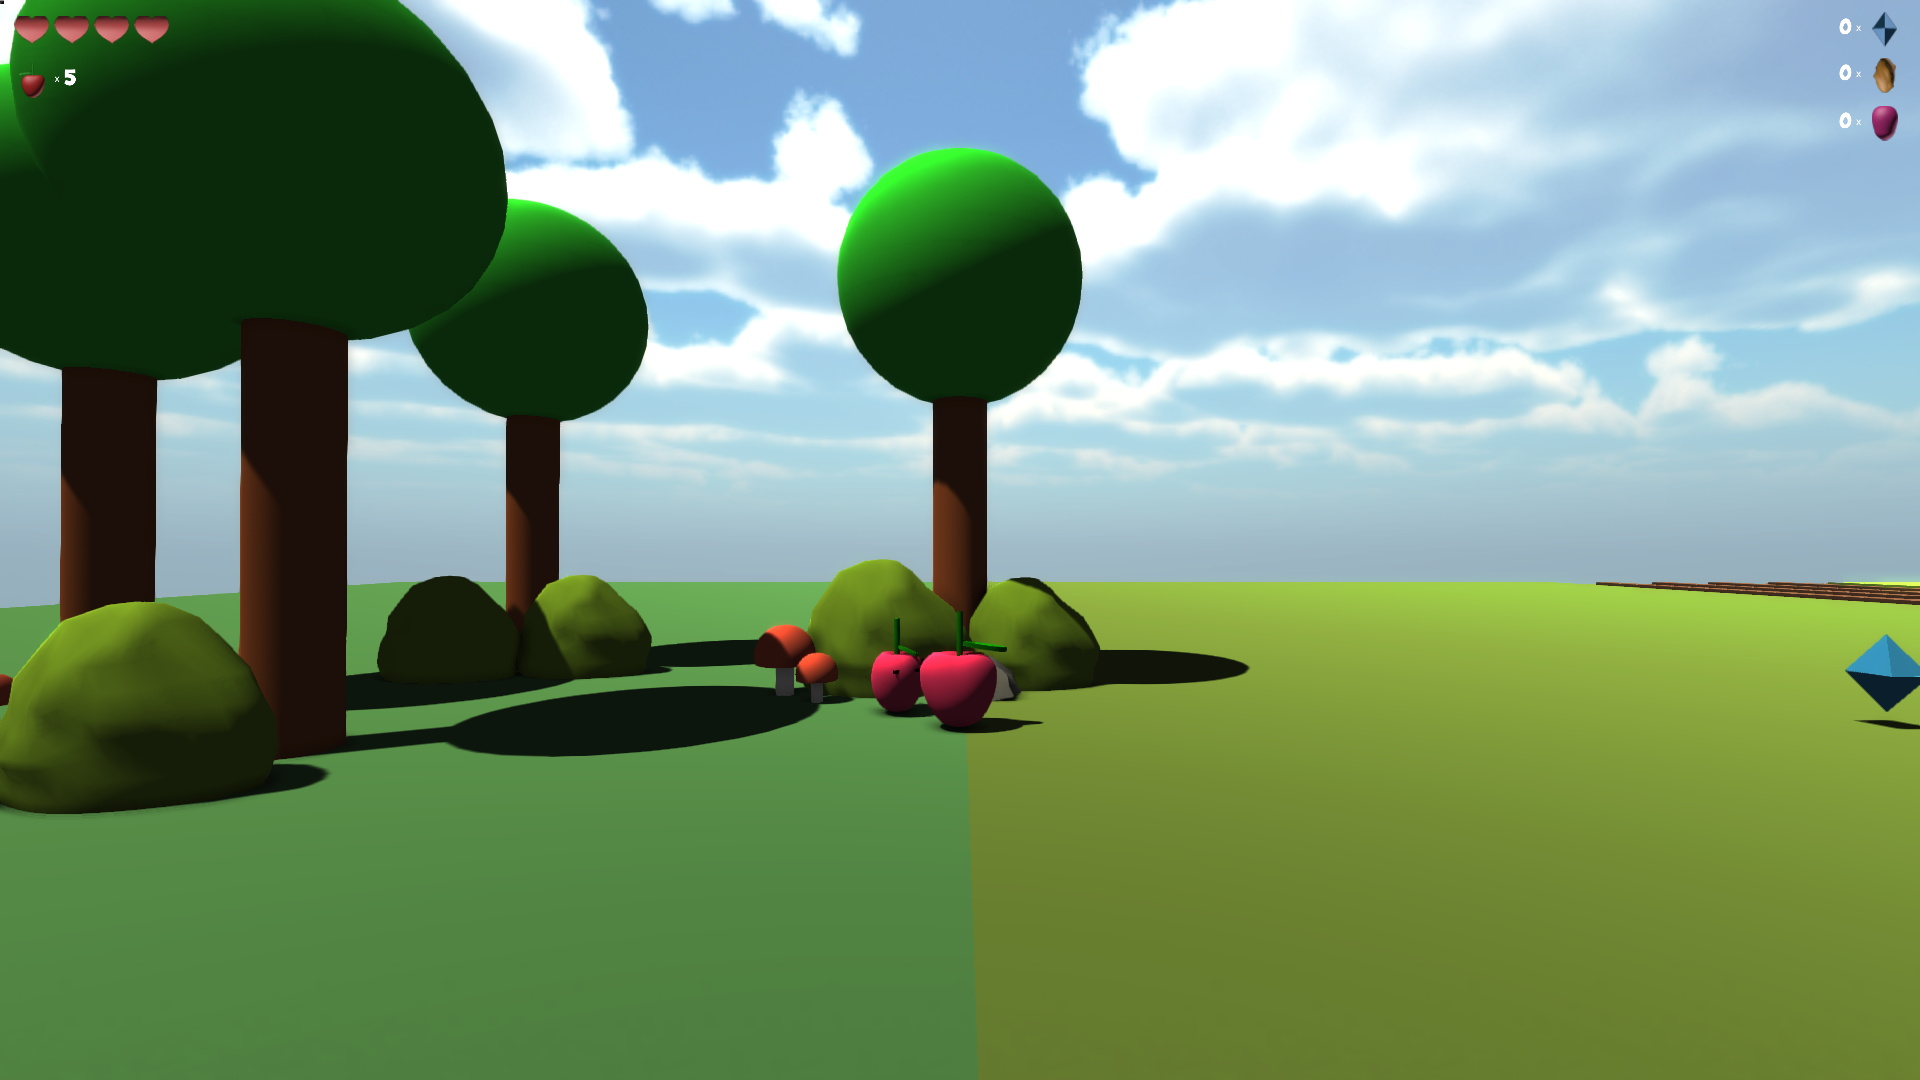
\includegraphics[page=1,width=0.98\linewidth]{Inhalt/Anhang/Screenshots/screenshot_1.png}}
	\end{center}	
	\caption[Am Fu�e des Baums]{Am Fu�e des Baums (Eigene Darstellung)}
	\label{fig:anhang_screenshots_level1_baum}
\end{figure}
%
\begin{figure}[H]
	\begin{center}
		\fbox{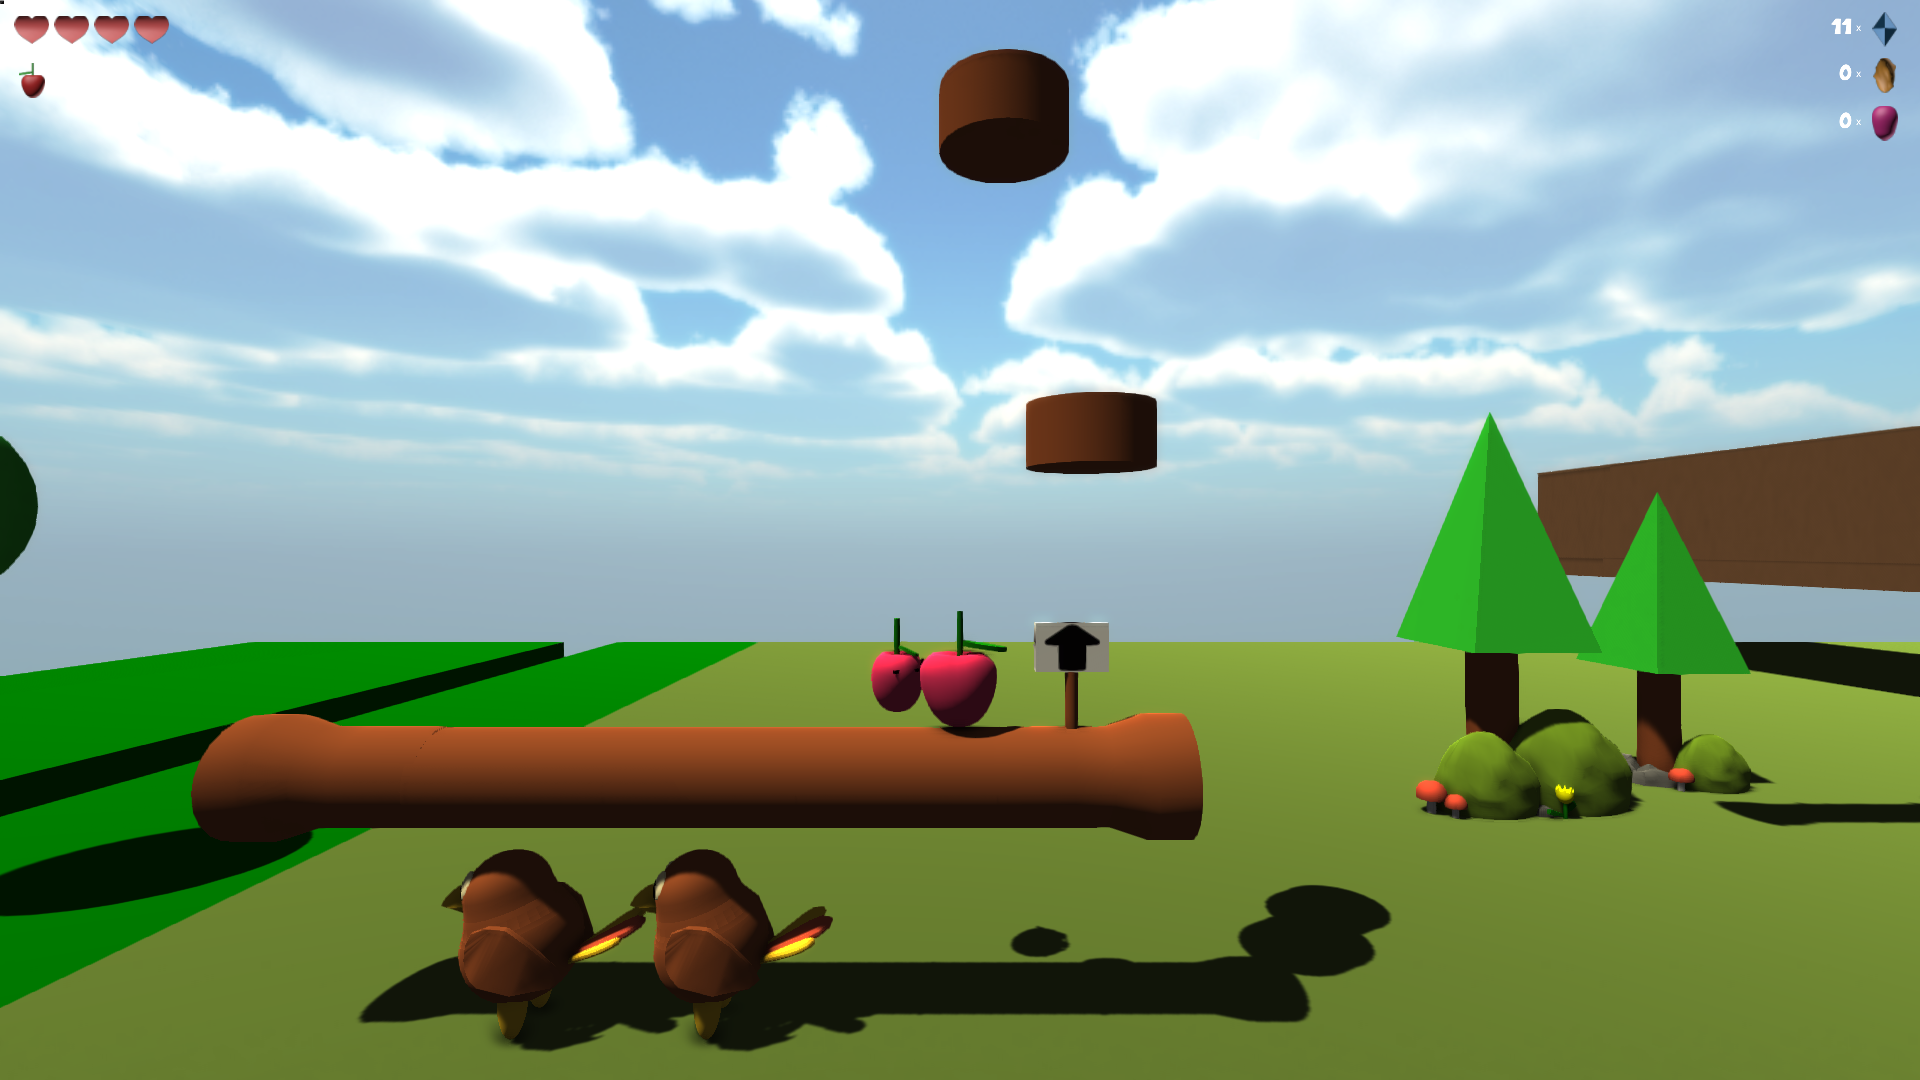
\includegraphics[page=1,width=0.98\linewidth]{Inhalt/Anhang/Screenshots/screenshot_4.png}}
	\end{center}	
	\caption[Versteckter Weg]{Versteckter Weg (Eigene Darstellung)}
	\label{fig:anhang_screenshots_level1_weg}
\end{figure}
%---------------------------------------------------------------------------------------------------------------------
\subsection{Der kaputte Brunnen}
\begin{figure}[H]
	\begin{center}
		\fbox{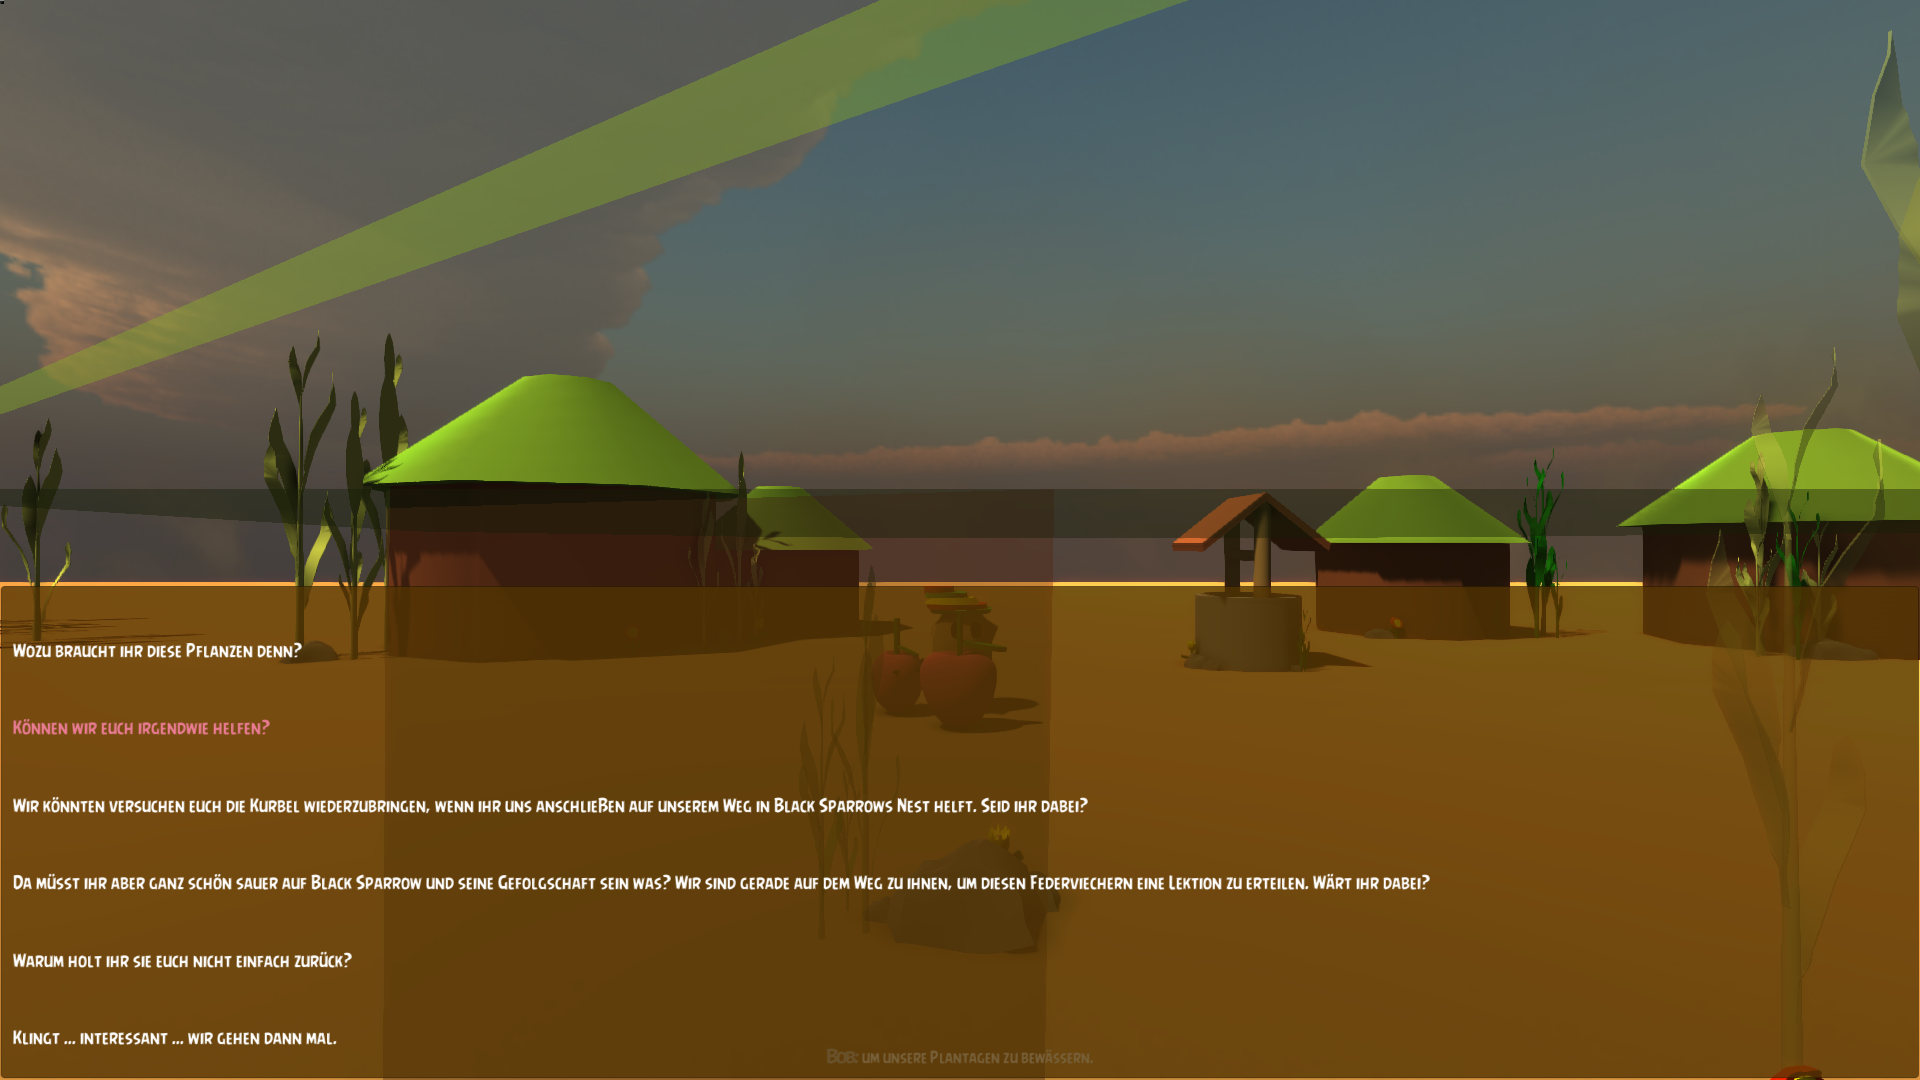
\includegraphics[page=1,width=0.98\linewidth]{Inhalt/Anhang/Screenshots/screenshot_8.png}}
	\end{center}	
	\caption[Unterhaltung mit Bob]{Unterhaltung mit Bob (Eigene Darstellung)}
	\label{fig:anhang_screenshots_level2_bob}
\end{figure}
\begin{figure}[H]
	\begin{center}
		\fbox{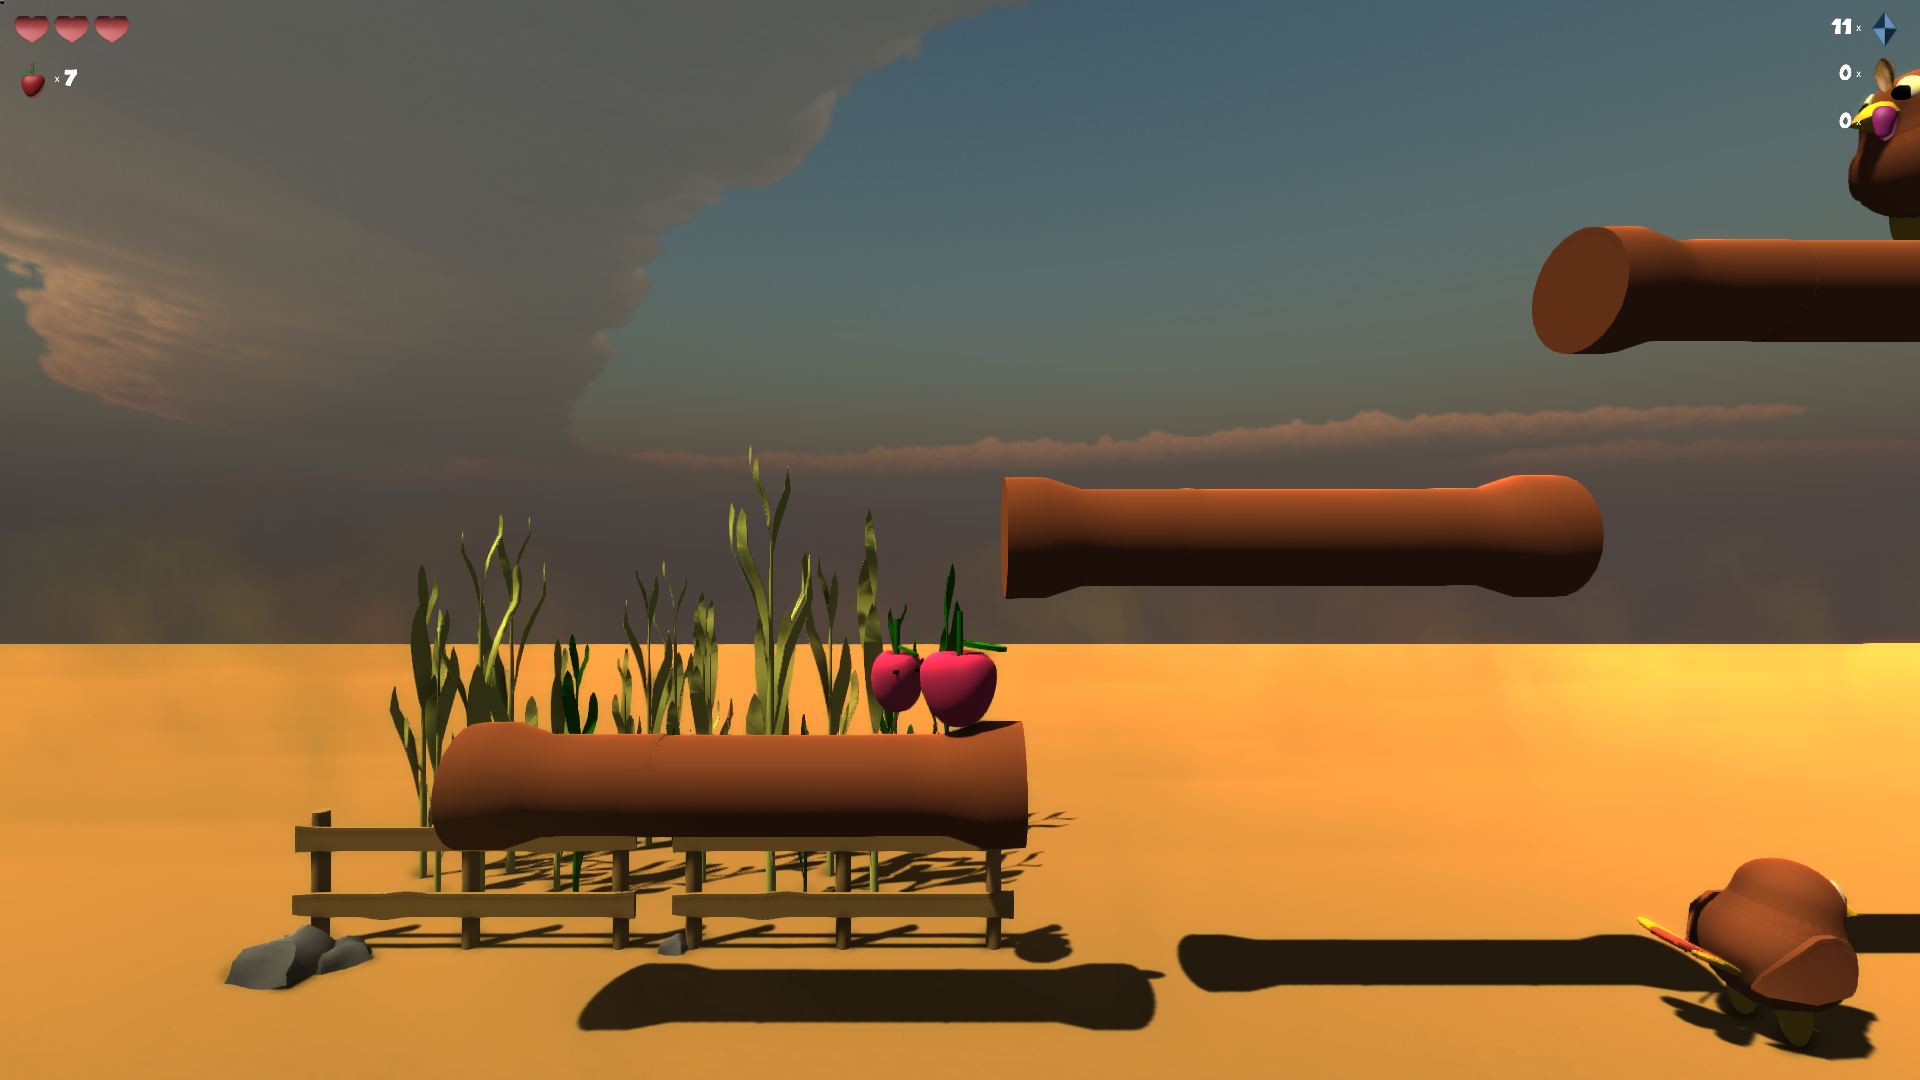
\includegraphics[page=1,width=0.98\linewidth]{Inhalt/Anhang/Screenshots/screenshot_9.png}}
	\end{center}	
	\caption[Pfad mit Hindernissen]{Pfad mit Hindernissen (Eigene Darstellung)}
	\label{fig:anhang_screenshots_level2_hindernisse}
\end{figure}
\begin{figure}[H]
	\begin{center}
		\fbox{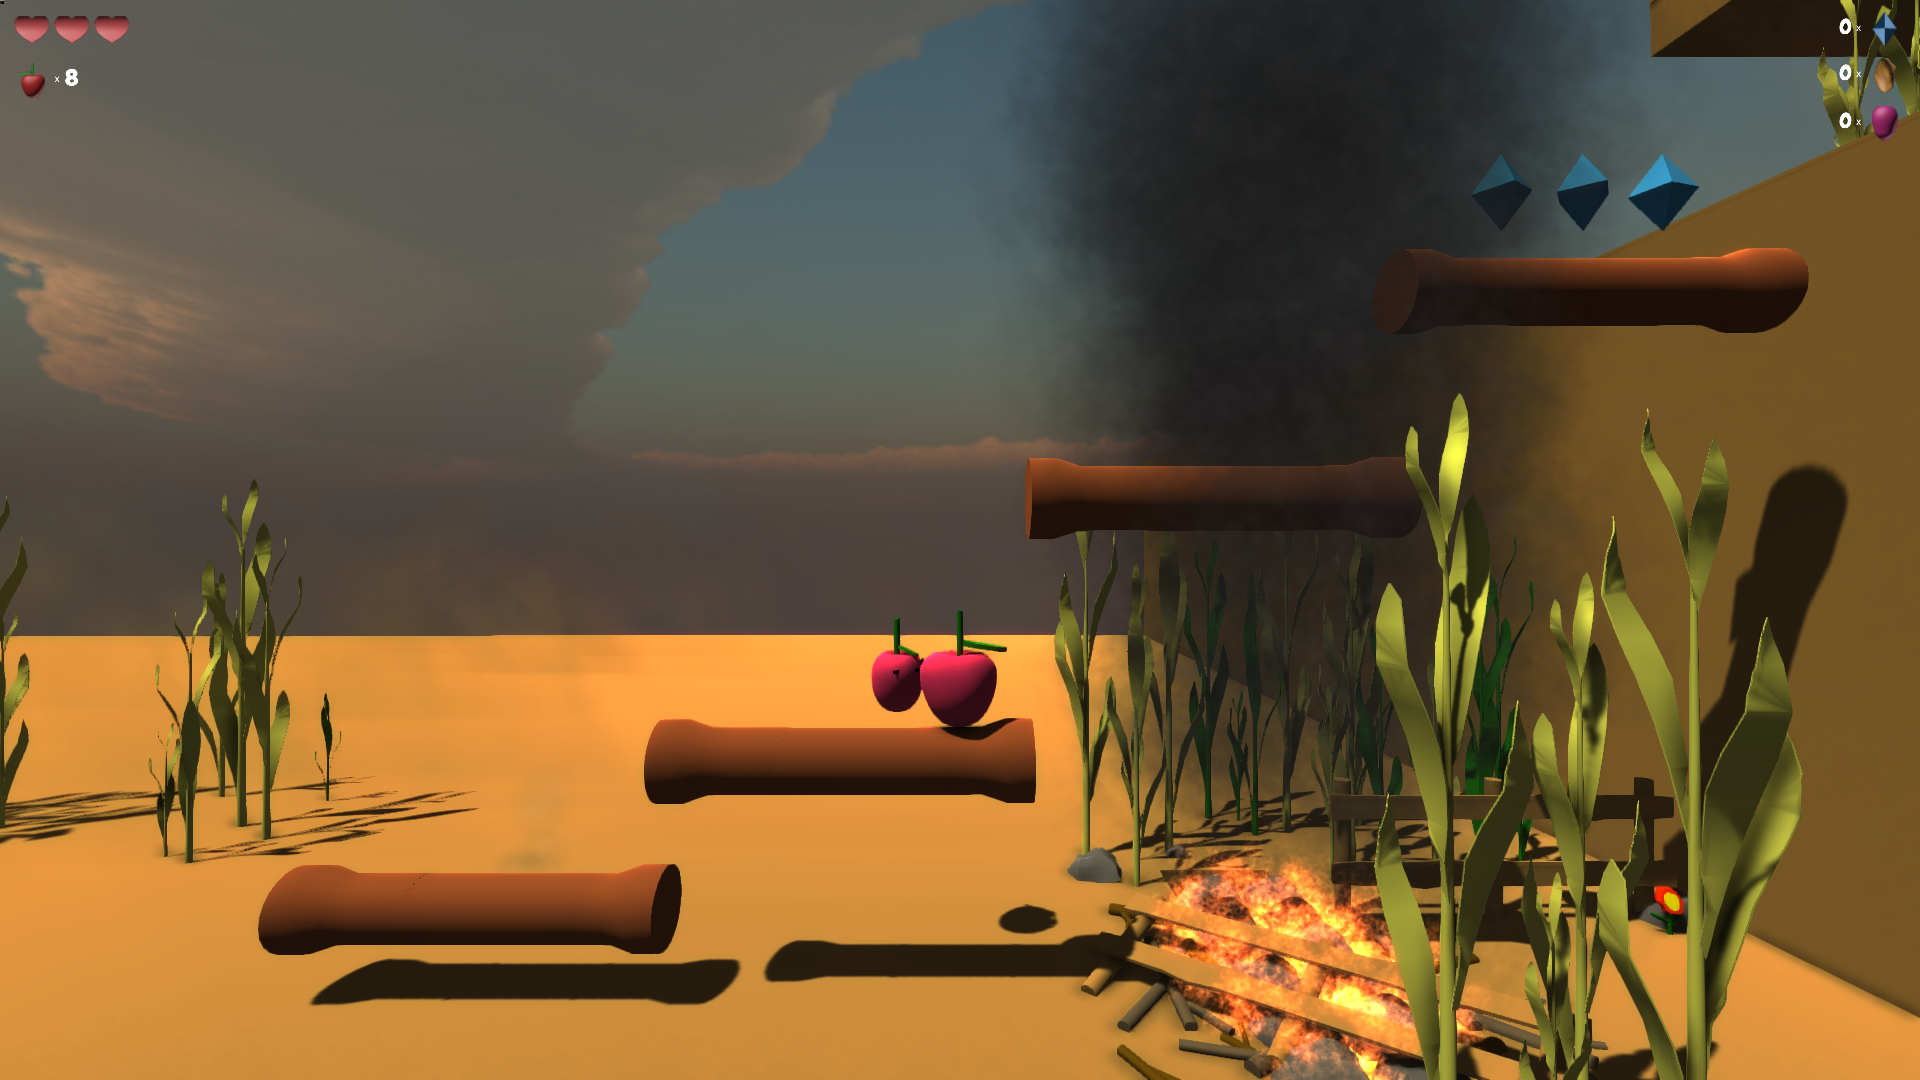
\includegraphics[page=1,width=0.98\linewidth]{Inhalt/Anhang/Screenshots/screenshot_12.png}}
	\end{center}	
	\caption[Eingest�rzte H�hle]{Eingest�rzte H�lle (Eigene Darstellung)}
	\label{fig:anhang_screenshots_level2_hoehle}
\end{figure}
%---------------------------------------------------------------------------------------------------------------------
\subsection{Der dunkle Wald} 
\begin{figure}[H]
	\begin{center}
		\fbox{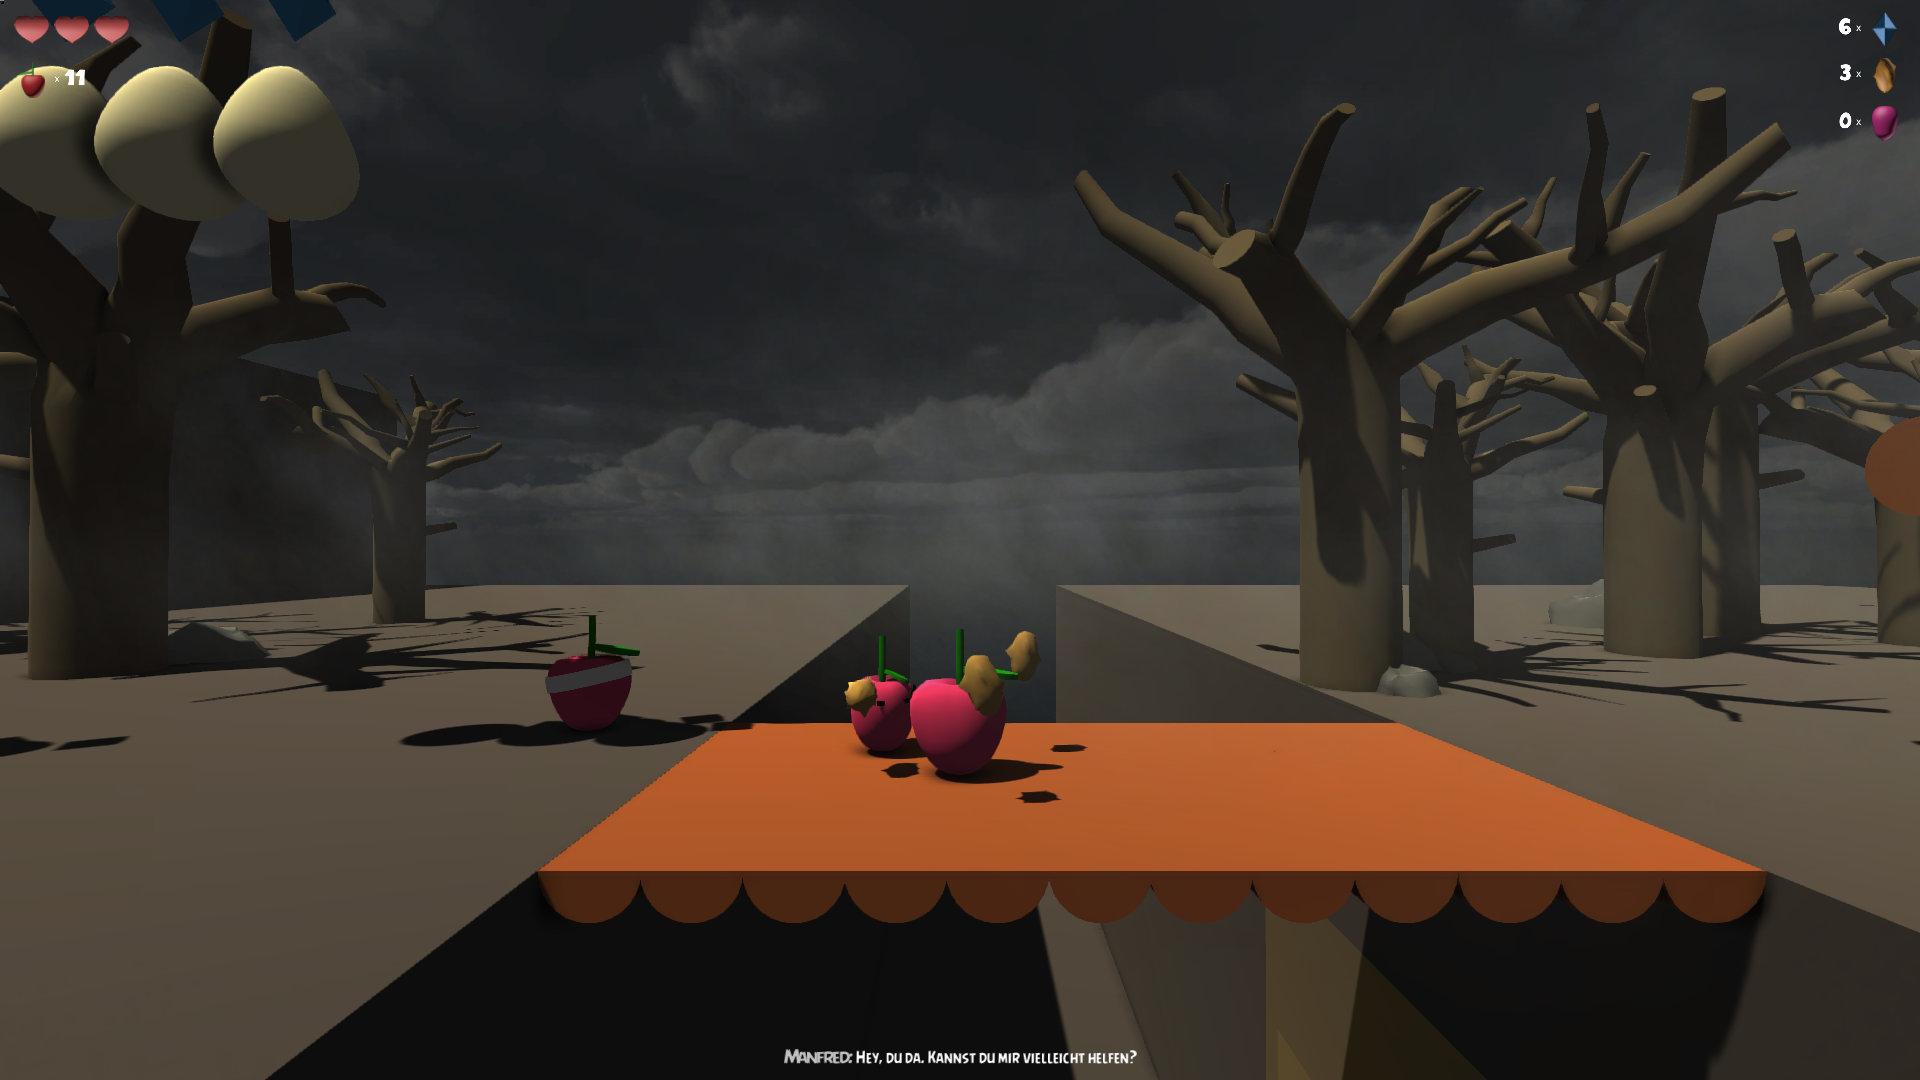
\includegraphics[page=1,width=0.98\linewidth]{Inhalt/Anhang/Screenshots/screenshot_22.png}}
	\end{center}	
	\caption[Unterhaltung mit Manfred]{Unterhaltung mit Manfred (Eigene Darstellung)}
	\label{fig:anhang_screenshots_level3_manfred}
\end{figure}
\begin{figure}[H]
	\begin{center}
		\fbox{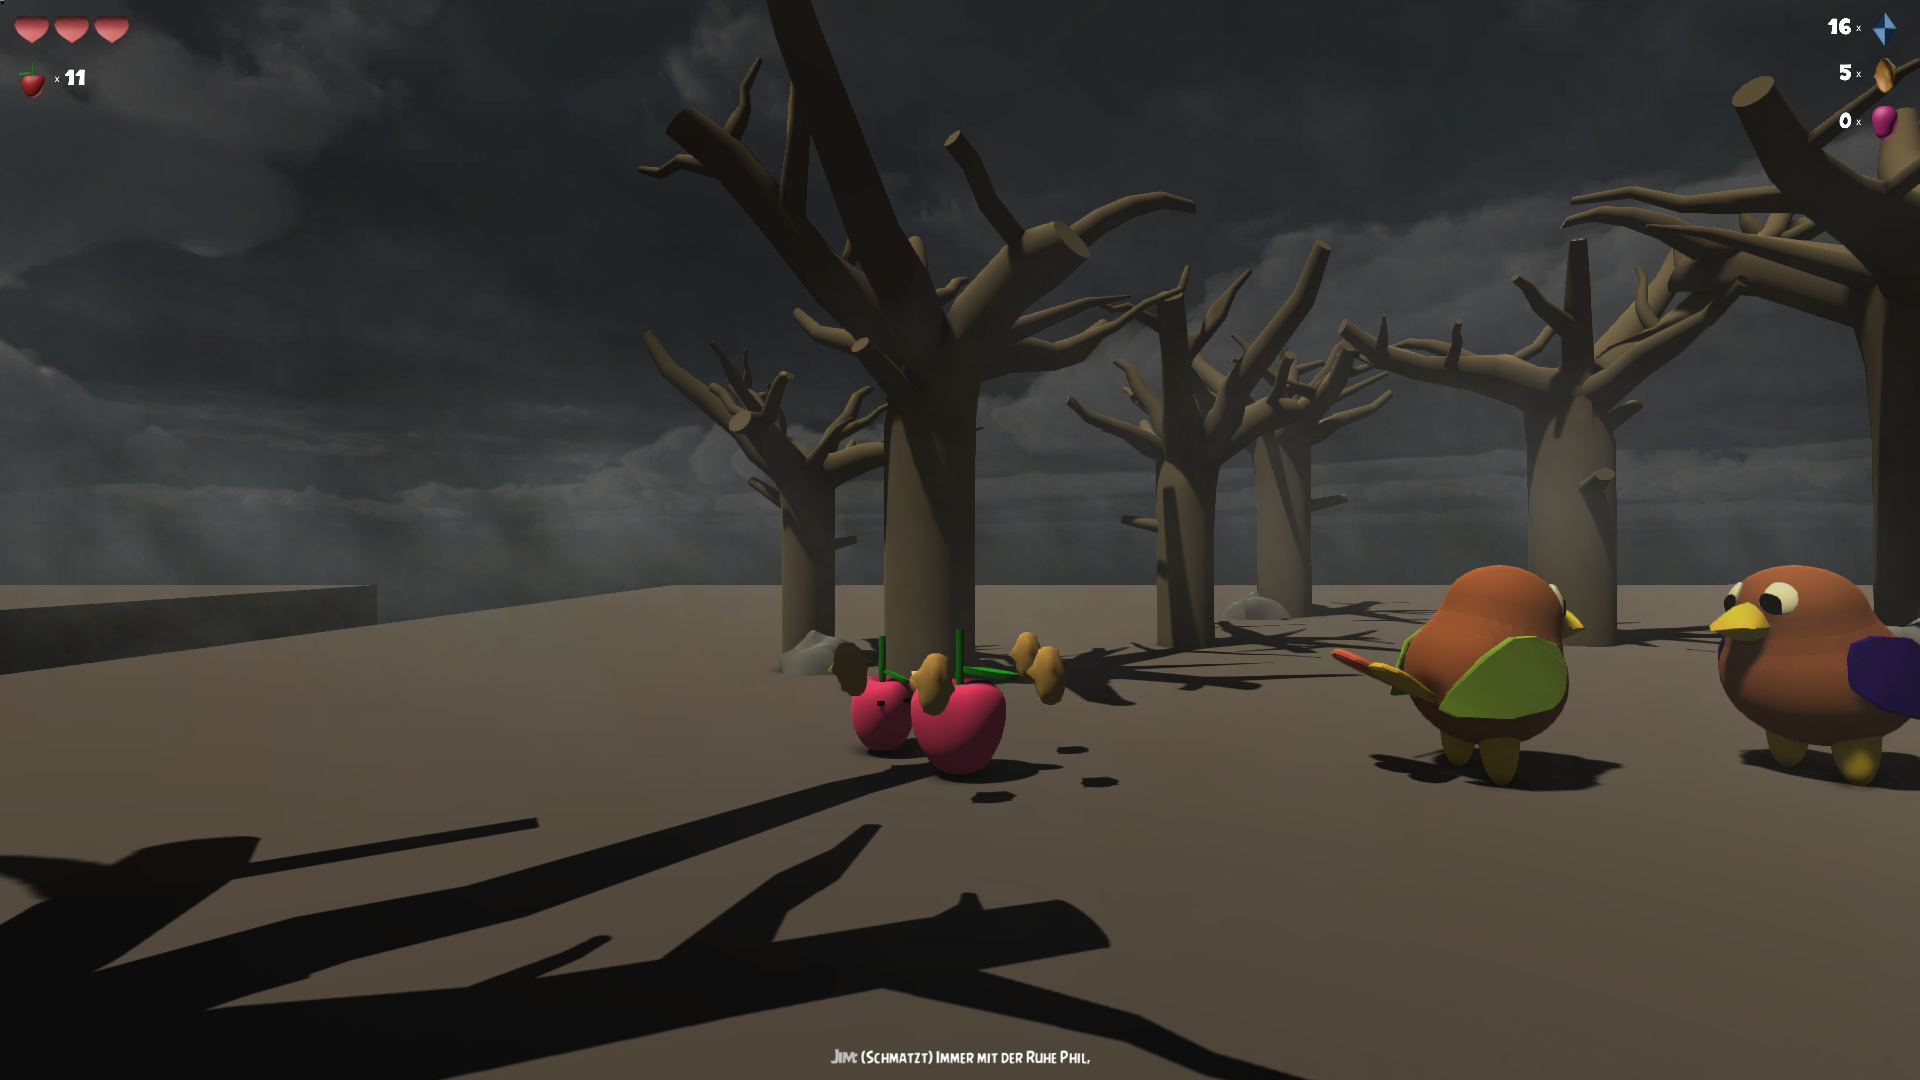
\includegraphics[page=1,width=0.98\linewidth]{Inhalt/Anhang/Screenshots/screenshot_24.png}}
	\end{center}	
	\caption[Verfolgung der Handlanger]{Verfolgung der Handlanger (Eigene Darstellung)}
	\label{fig:anhang_screenshots_level3_verfolgung}
\end{figure}
%---------------------------------------------------------------------------------------------------------------------
\subsection{Black Sparrow's Nest}
\begin{figure}[H]
	\begin{center}
		\fbox{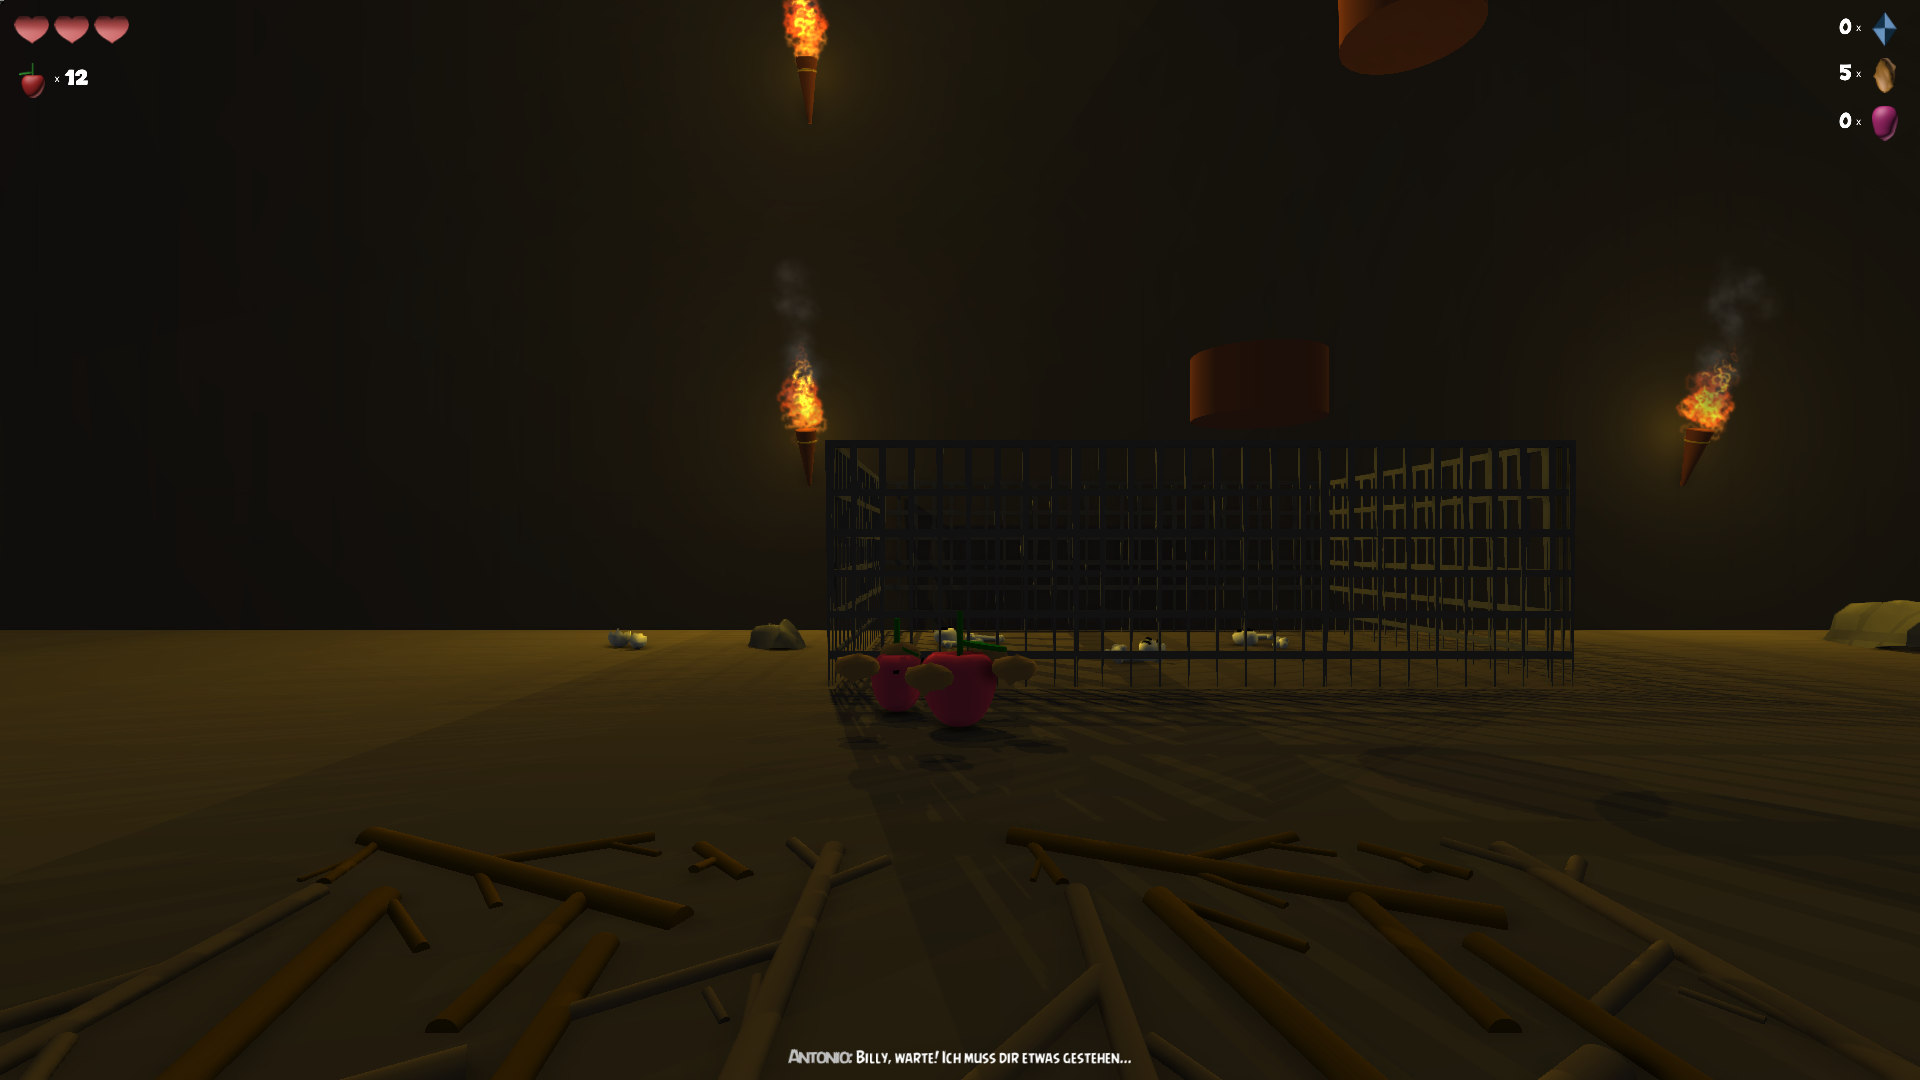
\includegraphics[page=1,width=0.98\linewidth]{Inhalt/Anhang/Screenshots/screenshot_30.png}}
	\end{center}	
	\caption[Antonios Gest�ndnis]{Antonios Gest�ndnis (Eigene Darstellung)}
	\label{fig:anhang_screenshots_level32_antonio}
\end{figure}
\showInContents	
\end{appendices}